\documentclass[tikz,border=5pt]{standalone}
\usepackage{tikz}
\usetikzlibrary{shapes.geometric, arrows.meta, positioning}

\begin{document}

\begin{tikzpicture}[
    node distance=2.5cm and 3cm,
    switch/.style={
        draw,
        rounded corners,
        minimum size=2cm,
        font=\sffamily,
        align=center,
        fill=gray!10
    },
    binary/.style={
        draw,
        circle,
        minimum size=2cm,
        font=\sffamily\Huge,
        align=center,
        fill=blue!10
    },
    arrow/.style={
        ->,
        >={Latex[length=3mm, width=2mm]},
        line width=1.5pt,
        color=black!70
    },
    label/.style={
        font=\sffamily\small,
        color=black!60
    }
]

% Main Title
%\node [font=\sffamily\Large\bfseries, yshift=1cm] (title) {Switch and Binary Representation};

% Physical Switch States
\node [switch] (off_switch) {
    \begin{tikzpicture}[scale=0.5]
        \draw[thick] (-1, 0) -- (-0.5, 0);
        \draw[thick] (0.5, 0) -- (1, 0);
        \draw[thick] (-0.5, 0) -- (0.3, 0.8); % Open switch arm
        \draw[fill=white] (-0.5, 0) circle (0.1);
        \draw[fill=white] (0.5, 0) circle (0.1);
    \end{tikzpicture}
    \\[1ex]
    \textbf{OFF}
};
\node [label, left=0.2cm of off_switch] {Physical State: Open};

\node [switch, right=of off_switch] (on_switch) {
    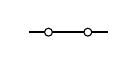
\begin{tikzpicture}[scale=0.5]
        \draw[thick] (-1, 0) -- (-0.5, 0);
        \draw[thick] (0.5, 0) -- (1, 0);
        \draw[thick] (-0.5, 0) -- (0.5, 0); % Closed switch arm
        \draw[fill=white] (-0.5, 0) circle (0.1);
        \draw[fill=white] (0.5, 0) circle (0.1);
    \end{tikzpicture}
    \\[1ex]
    \textbf{ON}
};
\node [label, right=0.2cm of on_switch] {Physical State: Closed};

% Section Title - Physical
\node [font=\sffamily\bfseries, above=0.5cm of off_switch, xshift=2.5cm] {Physical Switch State};


% Binary Representation
\node [binary, below=of off_switch] (binary_0) {0};
\node [label, below=0.2cm of binary_0] {Binary Value: 0};

\node [binary, below=of on_switch] (binary_1) {1};
\node [label, below=0.2cm of binary_1] {Binary Value: 1};

% Section Title - Binary
\node [font=\sffamily\bfseries, above=0.5cm of binary_0, xshift=2.5cm] {Binary Representation};

% Connecting Arrows
\draw [arrow] (off_switch) -- (binary_0) node[midway, left, font=\sffamily\small] {Maps to};
\draw [arrow] (on_switch) -- (binary_1) node[midway, right, font=\sffamily\small] {Maps to};

% Separator Line
\draw [dashed, color=black!30, line width=1pt] ([yshift=-1cm]off_switch.south west) -- ([yshift=-1cm]on_switch.south east);

\end{tikzpicture}

\end{document}